\documentclass[a4paper,12pt]{report}

\usepackage{alltt, fancyvrb, url}
\usepackage{graphicx}
\usepackage[utf8]{inputenc}
\usepackage{hyperref}
\usepackage[italian]{babel}
\usepackage[italian]{cleveref}

\title{Covid Simulation}

\author{Christian Ricci, Roberto Montalti, Juri Simoncini, Edoardo Savini}
\date{\today}

\begin{document}

\maketitle

\tableofcontents

\chapter{Analisi}

Il team si pone come obbiettivo lo sviluppo di una simulazione del Covid dentro l'università di Bologna. Lo scopo è poter permettere all'utente di visualizzare una possibile diffusione del Covid dentro l'università, attraverso una mappa virtuale della struttura. L'utente potrà inoltre modificare alcuni parametri della simulazione, per esempio potrà aggiungere nuove persone mentre la simulazione sta girando.

\section{Requisiti}

\subsection{Requisiti funzionali}
\begin{itemize}
\item L'applicazione permette di visualizzare una mappa dell'università, con una rappresentazione di alcune persone che si muovono all'interno della mappa.
\item Ci devono essere persone contagiate dal virus, e queste devono poter contagiare altre persone.
\item Le persone potranno indossare una mascherina che permetta a loro di abbassare la probabilità di contagio.
\item Durante la simulazione si potranno vedere quali persone sono state contagiate dal virus.
\item L'applicazione permette di iniziare una nuova simulazione con parametri differenti.
\item L'utente avrà la possibilità di girare all'interno della mappa e poter visualizzare come si diffonde il virus.
\item L'utente avrà anche la possibilità di aggiungere nuove persone alla simulazione, o di modificare alcuni parametri scelti all'inizio.
\end{itemize}

\subsection{Requisiti non funzionali}
\begin{itemize}
\item L'utente avrà la possibilità di "selezionare" una persona e poterla seguire automaticamente, semplicemente utilizzando il pulsante sinistro del mouse.
\item La simulazione dovrà avere diversi "preset" a disposizione, invece di dover scegliere le opzioni iniziali. Un preset è un insieme di opzioni iniziali per la simulazione.
\end{itemize}

\section{Analisi e modello del dominio}
Nella simulazione del Covid i soggetti principali sono le persone, le quali si muovono all'interno della mappa dell'università, ed il virus stesso, che gestisce le persone contagiate e cerca di contagiare nuove persone.

Le persone si muovono liberamente all'interno di una mappa, seguendo un apposito algoritmo di movimento. All'interno della simulazione c'è sempre almeno una persona contagiata dal virus, e c'è la possibilità che altre persone vengano contagiate se queste sono abbastanza vicine ad esso. Il meccanismo di infezione è gestito dal virus, che si occupa di guardare quali persone sono vicine ad una persona contagiata e di applicare a loro un algoritmo di infezione. Inoltre, ogni persona può indossare una mascherina, che può influenzare la possibilità di contagio.

La simulazione ha diversi parametri personalizzabili, quali il numero di persone, il numero di persone che non indossare una mascherina e il tipo di mascherina che ogni persona indossa.

Una delle principali difficoltà sarà dover trovare un algoritmo di movimento adatto alle persone, che sia realistico e non troppo banale. Un'altra difficoltà sarà nel gestire la diffusione del virus.

\chapter{Design}

\section{Architettura}

L'architettura di Covid Simulation si basa sull'MVC (Model - View - Controller) per quanto riguarda la parte della GUI (schermata iniziale, schermata di simulazione, schermata di pausa), e la visione ad alto livello del programma ma dentro alla simulazione stessa (dentro al Model) è stato usato un pattern differente, che si basa su un architettura a componenti seguita da alcuni videogiochi.
La classe Main funge da controller delle schermate: ad ogni aggiornamento di frame esso guarda in quale schermata è l'applicazione e va a chiamare un apposito metodo che per l'aggiornamento delle proprietà delle schermate.

Un apposito controller per la GUI, chiamato StartScreenController, gestisce le schermate iniziale e di pausa. Questo controller riesce a comunicare con il Main attraverso alcuni callback, e comunica con il controller della simulazione mandandogli direttamente i messaggi.

La view per la GUI non è stata fatto usando codice, bensì abbiamo utilizzato una libreria chiamata Nifty GUI, che permette lo sviluppo di GUI utilizzando XML. I bottoni della view sono solo legati ai metodi del controller: in questo modo, se volessimo cambiare la View, ci basterebbe assicurarci di chiamare i relativi metodi del controller per ogni bottone.

Il controller della simulazione è chiamato, appunto, Simulation ed esso gestisce il Model della simulazione, che comprende concetti quale il Virus e le persone. Esso ha disponibile un metodo per aggiornare tutte le persone, ed altri metodi per gestirle.

Ogni persona fa utilizzo di componenti, che gestiscono un solo concetto o sottosistema dell'engine: ad esempio, il MovementComponent gestisce il movimento della persona, mentre il GraphicsComponent gestisce tutto ciò che riguarda la grafica.

In figura è mostrata l'architettura ad alto livello dell'applicazione.

% qui ci vuole un bel uml immerdato

\section{Design dettagliato}

\subsection{Christian Ricci}

Io mi sono occupato per lo più di alcuni componenti del Model: Ad esempio, la classe della persona e alcuni dei suoi componenti. In particolare, io ho subito pensato, all'inizio del progetto, di creare un architettura a componenti per la persona, dato che sapevo che altrimenti la classe sarebbe diventata molto complessa, toccando varie parti dell'engine. Con un architettura a componenti, si va a scorporare queste parti, creando multiple classi che però diventano molto semplici, occupandosi di una sola cosa.

Assieme a Roberto Montalti ed Edoardo Savini ho creato il Movement Component e l'algoritmo di movimento: per l'algoritmo abbiamo pensato che la persona dovesse scegliere un punto casuale dentro la mappa, e grazie ad una libreria per l'AI offerta dal JMonkeyEngine la persona avrebbe trovato la strada migliore per arrivarci. Il Movement Component in sè deve prima richiedere la strada e poi iniziare a seguirla; la richiesta di una nuova strada da seguire può però essere molto costosa, dato che l'algoritmo per trovare la strada migliore è dispendioso. Questo si traduce in una serie di stati per il componente, e quindi abbiamo pensato di usare un pattern chiamato "State Pattern" per gestire tutti questi stati. Inoltre, abbiamo dovuto astrarre la richiesta della strada in una nuova classe, che facesse uso di una thread pool per gestire tutte le richieste di una nuova strada per tutte le persone.

In figura è mostrato un diagramma UML per il Movement Component.

Ho inoltre creato una prima versione della simulazione, che aveva semplicemente 2 metodi per inizializzarla e aggiornarla. Juri Simoncini ha poi esteso la simulazione, creando alcuni metodi per manipolare le persone.

Ho anche creato cose non legate al Model dell'applicazione: ad esempio ho creato una semplice gestione degli stati delle schermate nella classe Main, e ho creato un'interfaccia di callback per lasciare che il controller della GUI riesca a comunicare con la classe Main senza dover chiamare i suoi metodi direttamente: così facendo, si riesce a scorporare il controller della GUI dal resto dell'applicazione.

\subsection{Roberto Montalti}

Oltre ad aver contribuito all'algoritmo di movimento insieme a Christian Ricci ed Edoardo Savini, mi sono occupato di tutti gli aspetti grafici e fisici dell'applicazione e della gestione delle dipendenze che sono più in stretto contatto con il Jmonkey Engine.

In particolare per la gestione di medesimi, ho deciso di sfruttare il "Service Locator" pattern, con questa scelta di design è stato possibile separare in buona parte tanti aspetti dell'applicazione che non sono necessariamente legati al corretto funzionamento della sua logica.
Il motivo di questa decisione deriva dal momento in cui Io e Christian abbiamo notato che più andavamo avanti con gli sviluppi e più iniziavano a spargersi dipendenze su tutta l'applicazione.

Qui sotto riporto una semplice illustrazione dell'architettura appena menzionata.

\begin{figure}[h]
\centering{}
\includegraphics{./locator_uml.png}
\caption{Locator UML}
\label{img:Locator UML}
\end{figure}

\subsection{Juri Simoncini}
Io mi sono occupato dell'algortimo di infezione, la challenge principale erano capire su quali aspetti basarci per l'infezione, 
ho preferito utilizzare come parametri dell'algoritmo le proprietà della mascherina avendo cosi un'algoritmo semplice e leggero.
In seguito mi sono occupato del lato GUI: lato grafico e lato di controller.
La scelta principale da fare era decidere se suddividere i controller per schermata oppure tenerne uno per tutte le schermate.
Ho deciso di optare per la seconda soluzione dato che le feature da implementare non erano in grande quantità.
Però per alleggerire il codice ho deciso di suddividire le implementazioni dei metodi in varie classi suddivise per schermate.
Ho poi lavorato sulla simulazione per la manipolazione delle persone dato che mi era utile per le funzionalità del controller.

\subsection{Edoardo Savini}
Insieme a Christian Ricci e Roberto Montalti mi sono occupato del Movement Handler mentre personalmente ho effettuato il refactoring di altre classi e il testing delle stesse, incluso il testing automatizzato con GitHub Actions, usando le librerie jUnit per il testing e mockito per la creazione dei mock. Il testing è però incompleto a causa di alcune difficoltà riscontrate con alcune di esse, in quanto l'implementazione non permetteva lo stesso, anche invertendo il controllo.

\chapter{Sviluppo}

\section{Testing automatizzato}

Il testing automatizzato (non è possibile chiamarlo \emph{continuous integration} in quanto viene eseguita solo una compilazione con Gradle e i relativi test, senza la produzione di una release) è stato implementato per permettere a tutti i componenti di poter rifattorizzare il test e mettere a conoscenza gli altri componenti se era possibile effettuare il merge delle stesse sul branch principale. Sfrutta le GitHub Actions e si basa su un template fornito da GitHub stesso, poi adattato in quanto presentava alcuni problemi.

Durante il testing è stato utilizzato il framework jUnit per l'esecuzione dei test e le relative asserzioni e la libreria mockito per la creazione dei mock (le entità fantocce con cui abbiamo "ingannato" la classe sotto testing) permettendo l'isolamento delle classi le une dalle altre (cosa imprescindibile durante i test di unità).

Non sono stati creati test di integrazione a causa delle difficoltà riscontrate con il framework jMonkey Engine.

\section{Metodologia di lavoro}

\subsection{Metodologia in generale}

Abbiamo deciso di iniziare a sviluppare questo progetto con una fase di analisi, per capire esattamente cosa bisognasse fare, come potevamo suddividerci il lavoro e quali librerie potevamo utilizzare. Abbiamo presentato tutti le nostre idee riguardo al Model dell'applicazione. In retrospettiva la nostra fase di analisi potrebbe essere stata troppo corta, dato che ci siamo accorti più o meno a metà del progetto che l'engine non era particolarmente buono e abbiamo faticato molto per risolvere alcuni problemi legati alla librerie scelte.

Abbiamo deciso di suddividere in modo equo il lavoro, ma abbiamo anche pensato che sarebbe stato meglio collaborare insieme su alcuni componenti dell'applicazione che sono risultati più difficili da scrivere, ad esempio l'algoritmo di movimento della persona.

\subsection{Distributed Version Control System}

Per il DVCS è stato utilizzato git, dato che tutti i membri del team avevano esperienza solo su questo. Abbiamo creato una repository su github e abbiamo deciso di creare un branch per ogni membro del team. Questo alla fine ci è sembrato poco produttivo, data la difficoltà per ognuno di stare alla pari con le feature che altri membri creavano.

\subsection{Christian Ricci}

Sviluppo del Model dell'applicazione, in particolare la classe Simulazione, la classe Persona e alcuni dei suoi componenti e la classe Spawner. Sono stato in primo luogo a pensare all'architettura generale del Model e al design di alcuni dei suoi componenti. Ho inoltre contribuito ad fare il \textit{refactoring} di varie classi, tra cui il Virus e il controller della GUI.
Classi sviluppate singolarmente:
\begin{itemize}
\item Interfaccia Entity e classe PersonImpl
\item Spawner
\item MainMap
\end{itemize}

\subsection{Roberto Montalti}

Sviluppo di aspetti grafici e fisici dell'applicazione.

Per quanto riguarda gli aspetti grafici, ho pensato alla creazione dei creazione modelli tridimensionali, per questo ho fatto auisilio degli strumenti grafici blender e jmonkey terrain-editor, grazie a quest'ultimo ho ottenuto una Navigation-mesh della scena, utilizzata dal path-finder sfruttato nell'algoritmo di movimento.

Grazie a quest'ultima è stato possibile sviluppare un algoritmo di movimento il più semplice possibile, senza doverci preoccupare eccessivamente degli ostacoli che una persona può incontrare nel suo percorso,
dato che il Path Finder ci restituisce direttamente una lista di punti in maniera sequenziale, da inizio a fine percorso (il target).

La Navigation Mesh agisce come un grafo di fatto, dove cercare un percorso ottimale da un nodo dela grafo ad un altro.
In figura una possiamo notare: i triangoli che rappresentano i nodi del grafo, quindi le zone navigabili, e figure a più lati, che identificano gli ostacoli.

Classi sviluppate singolarmente:
\begin{itemize}
\item Locator e i suoi serivizi
\item PhysicsComponent
\item PersonPicker
\item Sceens e Controls, Models per la gui
\end{itemize}

\begin{figure}[h]
\centering{}
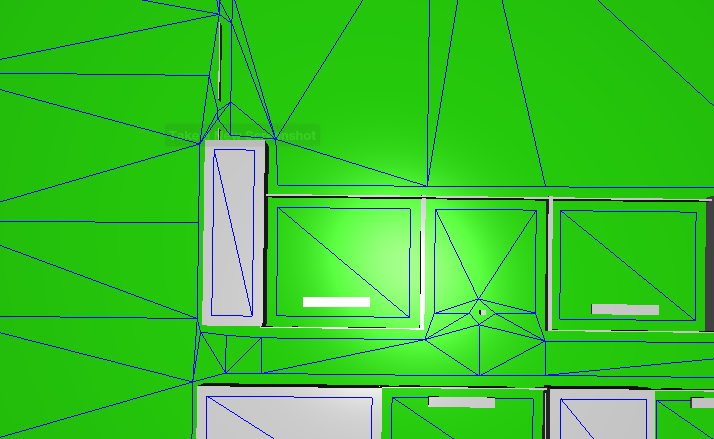
\includegraphics{./navmesh_obstacle.png}
\caption{Navigation Mesh}
\label{img:Navigation Mesh}
\end{figure}

Ho inoltre gestito tutti gli aspetti generali di rendering dell'ambientazione.

Per gli aspetti fisici invece ho gestito la parte di rilevazione delle collisioni e della rilevazione di prossimità di altre persone, dal punto di vista di un'altra.
Ho ottunuto successo in quest'ultima, grazie ad una "scatola di prossimità, che non è altro che un cubo invisibile e attraversabile, dove oggetti posso entrare e uscire, in questo caso persone.
Questo meccanismo sta alla base del funzionamento del virus.

In figura una semplice visualizzazione.

Ho inoltre pensato alla creazione del Virus e del PersonPicker.
Il modo in cui funziona il Virus è molto semplice si chiede ad una persona chi ha vicino in quel ciclo di esecuzione e si confronta il risultato con quello del ciclo precedente, questo è necessario per far sì che una persona tenti di infettarne un'altra solo una volta avvenuta la rilevazione della persona vittima nelle vicinanze.
Così facendo si garantisce l'integrità delle probabilità di contagio definite nell'infezione.

Il PersonPicker invece è una feature che ho deciso spontaneamente di implementare, per arrichire quella che è l'esperienza utente.
Questo segue una logica molto semplice, si prende la direzione della telecamera, in seguito si proietta una retta in quella direzione e se questa entra in collisione con una persona, si posiziona la telecamera sopra la persona finchè non ci si stacca da essa.

Oltre a questo ho contribuito al miglioramento della struttura dei package dell'applicazione e alla ristrutturazione del suo codice in svariate classi.

\subsection{Juri Simoncini}
Lato GUI sia a lato grafico che a lato logico utilizzando la libreria Nifty GUI.

L'implementazione grafica si trova dentro al file screen.xml che poi viene passato allo StartScreenController, il controller della nostra GUI.
Tutta l'interfaccia è stata organizzata per schermate, quindi è presente per ogni schermata (Start, Commands, Edit, Pause) uno screen nel file screen.xml.
Lo StartScreenController presenta al suo interno tutti i metodi che vengono chiamati dai vari screen (bottoni, pulsanti, textField...).
Per l'edit screen ho implementato una classe chiamata EditComponent con all'interno la logica per i metodi utili allo StartScreenController, stessa cosa ho attuato per il load screen con il loadComponent.

Mentre per il testo presente nell' HUD ho optato per un oggetto separato dal controller, per non sovraccaricarne il lavoro, chiamato HudText.
Il testo presente così riesce ad aggiornarsi in tempo reale grazie al metodo SimpleUpdate presente nel Main.
L'algoritmo di infezione che viene utilizzato per infettare le varie persone presenti nella mappa.
L'algoritmo si basa sulle dell'oggeto mask: Protection (FP1, FP2, FP3) e Status (UP, DOWN).
Ho preferito assegnare più rilevanza allo status in base anche alle esperienze nella vita reale dato che una mascherina abbassata avrà un effetto maggiore sulla trasmissione del virus.

Quindi lo status in percentuale ha un 70\% di rilevanza mentre la protection il restante 30.
Perciò ho pensato alla trasmissibilità dell'infezione come una scala di valori da 0 a 100 in cui, per esempio, se la mascherina è abbassata ed è di tipo FP1 le probabilità di trasmissione è pari a 100.

Per rappresentare la casualità del contagio viene estratto un valore random da 0 a 100 e se questo è minore del valore della trasmissibilità calcolato la persona viene contagiata, quindi maggiore è il valore di trasmissibilità maggiori sono le porbabilità di essere contagiato.

\subsection{Edoardo Savini}

Sviluppo del Movement Handler e del testing.
Classi sviluppate singolarmente:
\begin{itemize}
    \item \emph{PathManager};
    \item \emph{StuckManager};
    \item tutte le classi di testing.
\end{itemize}

\section{Note di sviluppo}

\subsection{Christian Ricci}

Per quanto riguarda aspetti più avanzati del linguaggio:
\begin{itemize}
\item Thread Pool: un uso di una thread pool è stato fatto dentro al Movement Component per gestire le richieste di nuove strade.
\item Programmazione funzionale e lambda: l'interfaccia di Callback dentro il GUI controller è funzionale, per permettere di scrivere semplici lambda.
\item Generici: l'interfaccia di callback è anche generica, per permettere di registrare un qualunque callback.
\end{itemize}

Per quanto riguarda le librerie:
\begin{itemize}
\item JMonkeyEngine: engine utilizzato per il Model dell'applicazione;
\item JMonkeyEngine AI: libreria utilizzata all'interno dell'implementazione del Movement Component;
\end{itemize}

\subsection{Roberto Montalti}

\begin{itemize}
\item JMonkeyEngine: engine utilizzato per il Model dell'applicazione;
\item JMonkeyEngine AI: libreria utilizzata all'interno dell'implementazione del Movement Component;
\item Bullet: libreria nativa C++, per la gestione di spazi fisici;
\item Thread Pool: un uso di una thread pool è stato fatto dentro al Movement Component per gestire le richieste di nuove strade;
\item Jmonkey Terrain Editor e Blender: per la creazione di modelli e per la Navigation Mesh; 
\end{itemize}

\subsection{Juri Simoncini}

\begin{itemize}
\item JMonkeyEngine: engine utilizzato per tutta l'applicazione.
\item Nifty-gui: libreria utilizzata in tutto lo sviluppo della gui.
\item Uso di lambda expressions.
\end{itemize}

\subsection{Edoardo Savini}

\begin{itemize}
    \item \emph{jUnit}: il framework utilizzato per i test;
    \item \emph{mockito}: il framework che permette di creare dei mock delle interfacce e delle classi, permettendo di isolare i singoli componenti nei test d'unità.
\end{itemize}

\chapter{Commenti finali}

\section{Autovalutazione e lavori futuri}

\subsection{Christian Ricci}

Mi sento soddisfatto del lavoro fatto per questo progetto; sin dall'inizio ho cercato di dare contributi fondamentali, ma soprattutto ho cercato di esporre le mie idee al gruppo e cercato di migliorare alcune parti della struttura del progetto che secondo me erano fatte male.

Sono però leggermente dispiaciuto del fatto che non sono riuscito ad implementare alcune delle mie idee a causa di alcuni ritardi, ma anche a causa del fatto che non ho contribuito linearmente al progetto: più o meno verso metà non sono più stato molto partecipe e penso che forse il progetto ne abbia sofferto.

Sono stato contento del mio team, in particolare del mio compagno Roberto Montalti, con cui condividevo di più le mie idee e con cui ho collaborato su alcune classi. Questo non è stato il mio primo progetto, però è sicuramente stato il primo progetto con cui ho avuto a che fare con più persone: io ho sempre lavorato da solo ai miei progetti, quindi aver lavorato insieme mi ha fatto capire quanto può essere difficile alcune volte comunicare con il team e coordinarsi sul da fare.

Sono abbastanza contento del lavoro finale, anche se, come ho detto prima, sono stato deluso dal fatto che non sono riuscito ad implementare alcune mie idee. D'altro canto, penso che il risultato finale sia più che soddisfacente, anche tenendo conto del tempo trascorso.

\subsection{Roberto Montalti}

Tenendo in conto gli ostacoli incontrati nel corso di questi mesi e il tempo impiegato per arrivare conoscere a fondo l'engine, mi sento soddisfatto del risultato finale ottenuto, anche se come progetto a parer mio avrebbe potuto offrire di più.

Sono soddisfatto inoltre del lavoro svolto dal mio team, che ha fatto il possibile per mantenere la promessa di portare a termine questo progetto in uno stato presentabile e apprezzabile, ho capito quanto sia importante essere coordinati in squadra e ancor più quanto sia importante una costante presenza da parte di tutti, anche se i partecipanti più attivi e presenti eravamo spesso io e il mio compagno Christian Ricci, con cui ho condiviso e implementato gran parte delle idee sorte durante lo sviluppo del progetto.   

Questo per me è il primo progetto di questa portata, in cui mi trovo a lavorare con più di due persone e devo dire che l'organizzazione di gruppo viene spesso sottovalutata, da ora ritengo sia una priorità stabilire con largo anticipo come suddividire il carico di lavoro in ragioni di tempo e abilità per ogni membro del gruppo.

Ho sicuramente imparato molte altre cose interessanti e importanti, programmare in una manierà più consapevole e l'organizzazione di squadra sono state sicuramente alcune di queste.

\subsection{Juri Simoncini}

Avrei potuto sicuramente fare di più ma per vari problemi non sono riuscito a mettere in atto tutti gli insegnamenti compresi a lezione soprattutto per quanto riguarda l'utilizzo del pattern MVC nella GUI che sarebbe potuto essere attuato in maniera migliore.

D'altro canto ritengo però di averci messo tutto l'impegno possibile per aiutare i miei colleghi nello sviluppo dell'applicazione e nello sviluppo portato avanti da me.

In conclusione ritengo che lo sviluppo di questa applicazione abbia ampliato le mie conoscenze facendomi conoscere un engine tutto nuovo e perciò avendo acquisito una nuova skill.

\subsection{Edoardo Savini}

\section{Difficoltà incontrate e commenti per i docenti}

\subsection{Christian Ricci}

Sono stato abbastanza contento del percorso che si è fatto durante il corso: ho appreso molti argomenti che a mio parere sono molto interessanti ed utili, ad esempio lambda e stream. I professori sono stati molto bravi a spiegare i vari argomenti del corso, e io personalmente son sempre riuscito a seguire bene ogni lezioni: nessun argomento mi è sembrato molto difficile da apprendere.

Avrei però voluto un po' di spiegazione in più riguardo ad alcuni argomenti di laboratorio, in particolare il tool Gradle, che è stato spiegato molto velocemente a mio parere, e che forse avrebbe fruttato spendere qualche ora in più ad imparare come usarlo, specialmente perchè penso che in un contesto lavorativo il build system di un progetto dovrebbe conosciuto quanto il linguaggio stesso. Avrei voluto anche qualche spiegazione in più sullo Unit Testing e forse anche una breve introduzione sul CI.

\subsection{Roberto Montalti}

% sku qui ci vanno i commenti per il corso
Buona parte di noi, ha avuto problemi non indifferenti nell'essere costanti con lo sviluppo, principalmente per motivi sia lavorati che universitari.
Questo è il motivo per cui magari alcuni abbiano partecipato al progetto con meno costanza, rispetto ad altri.

\subsection{Juri Simoncini}

\subsection{Edoardo Savini}

\appendix

\chapter{Guida utente}

All'avvio dell'applicazione si aprirà una schermata iniziale da cui si possono selezionare alcune opzioni iniziali e poi iniziare la simulazione.

\begin{figure}[h]
\centering{}
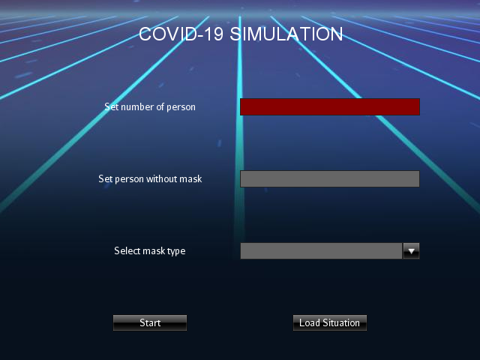
\includegraphics{1.png} 
\caption{La schermata iniziale.}
\label{img:startscreen}
\end{figure}

Spiegazione delle opzioni:
\begin{itemize}
\item Numero di persone: il numero totale di persone;
\item Numero di persone senza mascherina: il numero di persone che non utilizzerano una mascherina;
\item Tipo di mascherina: questo indica il tipo di protezione che le mascherine useranno. Si può scegliere tra 3 opzioni: FP1, FP2, FP3;
\end{itemize}

Selezionando il pulsante "Start" si inizia subito la simulazione con le opzioni selezionate. Altrimento, selezionando "Load simulation", si accede alla schermata dei preset.

\begin{figure}[h]
\centering{}
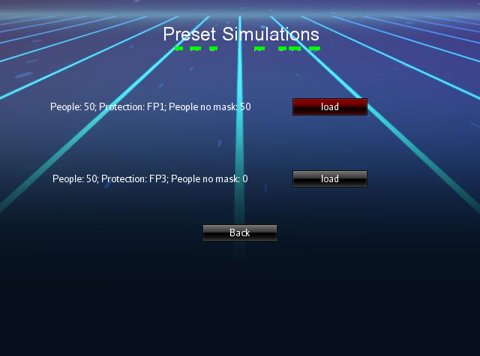
\includegraphics{2.png} 
\caption{I preset della simulazione.}
\label{img:preset}
\end{figure}

Qui si ha la possibilità di selezionare alcuni preset, che comprendono opzioni pre-selezionate.

Qualunque metodo si scelga per iniziare, si arriverà subito alla schermata della simulazione.

\newpage

\begin{figure}[h]
\centering{}
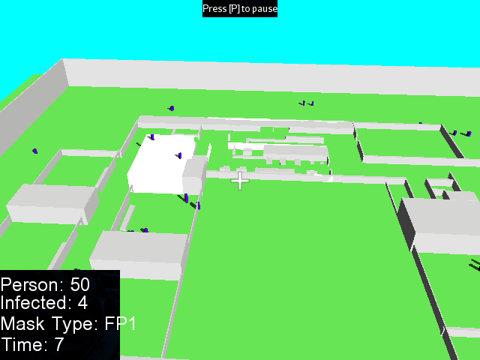
\includegraphics{3.png} 
\caption{La schermata della simulazione.}
\label{img:scene}
\end{figure}

Dentro la simulazione, si può girare liberamente per la mappa usando i pulsanti WASD. Inoltre, cliccando su una persona con il pulsante sinistro del mouse, si andrà in visualizzazione persona: la camera si muoverà secondo la persona e non si potrà più girare liberamente. Per ritornare in visualizzazione globale, basta premere il pulsante destro.

\newpage

Premendo P si andrà nella schermata di pausa.

\begin{figure}[h]
\centering{}
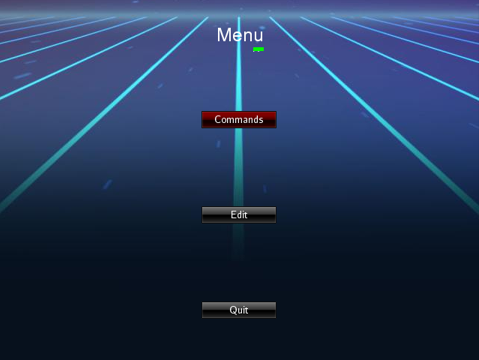
\includegraphics{4.png} 
\caption{La schermata di pausa.}
\label{img:pause}
\end{figure}

Nella schermata di pausa si può:
\begin{itemize}
\item Visualizzare i comandi della simulazione;
\item Cambiare alcuni parametri della simulazione;
\item Uscire dal programma;
\end{itemize}

\newpage

\begin{figure}[h]
\centering{}
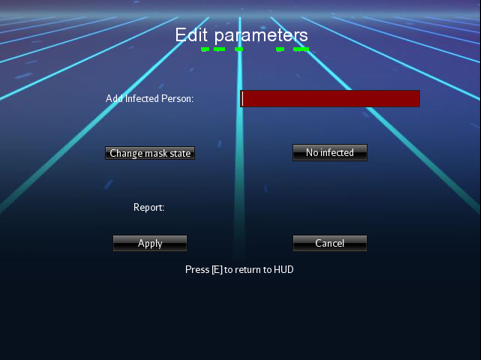
\includegraphics{5.png} 
\caption{Opzioni della simulazione.}
\label{img:edit}
\end{figure}

In questa schermata si possono cambiare alcuni parametri. Più nello specifico:
\begin{itemize}
\item Aggiungere nuovi infetti: questa opzione va a cambiare persone esistenti, non ne aggiunge di nuove;
\item Cambiare lo stato delle mascherine (pulsante "Change mask state"): le persone che non indossavano la mascherina adesso la indosserano, e viceversa;
\item Curare ogni person (pulsante "No infected"): va a curare ogni persona dall'infezione. Ci sarà comunque almeno una persona infettata;
\end{itemize}

Il pulsante "Apply" va ad applicare queste opzioni; il pulsante "Cancel" annulla le modifiche.

\end{document}
